\documentclass[a4paper]{article}

\usepackage[english]{babel}
\usepackage[utf8]{inputenc}
\usepackage{graphicx}
\usepackage[colorinlistoftodos]{todonotes}

\title{Rotating Object}

\author{Maurice Leavell}

\date{September 9, 2014}

\begin{document}

\begin{figure}
\centering
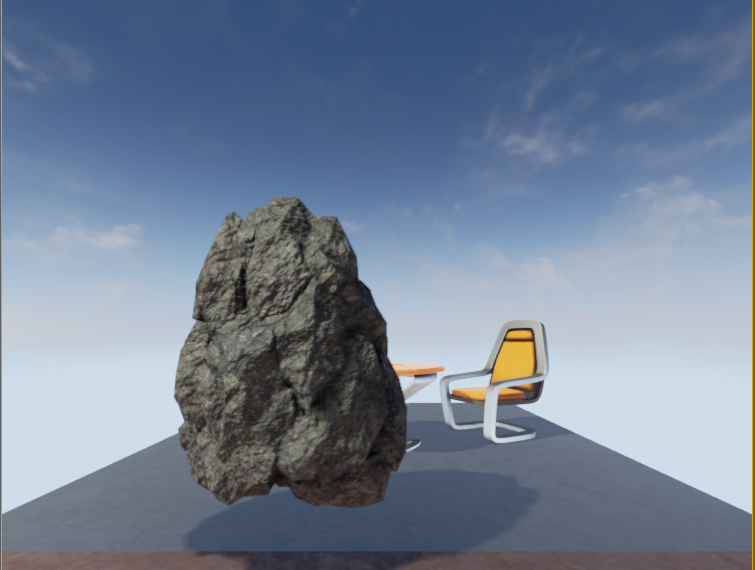
\includegraphics[width=0.4\textwidth]{rotating_Object.png}
\end{figure}

\maketitle

\section{Summary}

This level blueprint was created by every student in the independent study as a starting excercise. The goal of the blueprint was to make an actor of the student's choosing rotate yaw - wise at a rate of their choosing between 1 and 179 degrees. There were difficulties considering mutliple members had no previous experience with the Blueprint Visual Scripting Language, but considering the simplicity of the excercise it was easy to explain features on the fly.

\section{Code Snapshot}

\textbf{NOTE:} Due to the nature of level blueprints, we can not provide complementary code for this excercise. Screenshots will be all that is offered.

\begin{itemize}
\item rotatingObjectLevelBlueprint.PNG
\item rotatingObjectLevelBlueprintEventGraph.png
\item rotatingObjectLevelBlueprintVariables.png
\end{itemize}

\end{document}